\subsubsection{Three-tier client/server architecture}
Our system is based on a client/server architecture with three layers.
Presentation, application and data access are physically separated repectively in Mobile App, Application Server and Database server, as shown in the Deployment View \ref{deploysect}.

We choose this kind of architecture in order to have a modular system, whick keeps the client application very light and all the heavy computation is done on the server side. Moreover we separated physically the database from the application server, to increase scalability and security, and it's also possible to use a distribuited database.


\subsubsection{Clean Architecture}
As already introduced, each part of our system will use the Clean Architecture, proposed by Robert C. Martin. We apply this architecture both on the Client (Mobile application) and in the Application Server.

\begin{figure}[H]
\centering
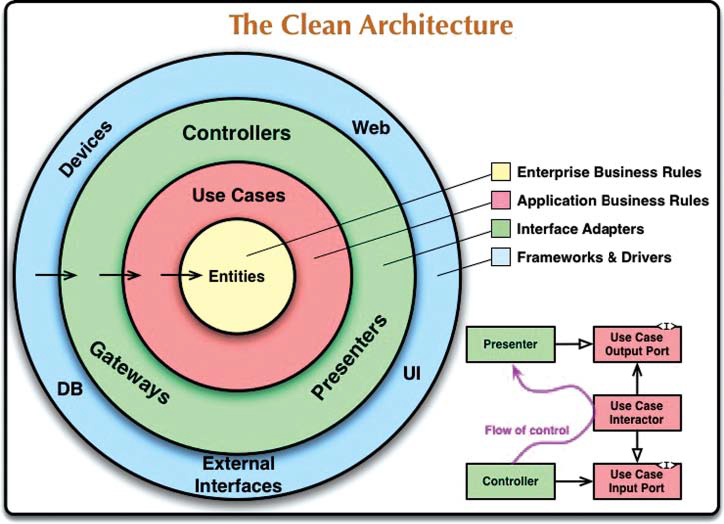
\includegraphics[width=.7\textwidth]{Images/cleanArchi.pdf}
\caption{\label{fig:cleanArchi} Clean Architecture \cite{clean} p. 203}
\end{figure}

\paragraph{Dependency Rule}
"The concentric circles in Figure \ref{fig:cleanArchi} represent different areas of software. In general, the further in you go, the higher level the software becomes. The outer circles are mechanisms. The inner circles are policies.
The overriding rule that makes this architecture work is the Dependency Rule:
\textit{Source code dependencies must point only inward, toward higher-level policies.}
Nothing in an inner circle can know anything at all about something in an outer circle. In particular, the name of something declared in an outer circle must not be mentioned by the code in an inner circle. That includes functions, classes, variables, or any other named software entity." \cite{clean}

\paragraph{Entities}
"Entities encapsulate enterprise-wide Critical Business Rules. An entity can be an object with methods, or it can be a set of data structures and functions. It doesn’t matter so long as the entities are the business objects of the application. They are the least likely to change when something external changes. For example, you would not expect these objects to be affected by a change to page navigation or security. No operational change to any particular application should affect the entity layer." \cite{clean}

\paragraph{Use Cases}
"The software in the use cases layer contains application-specific business rules. It encapsulates and implements all of the use cases of the system. These use cases orchestrate the flow of data to and from the entities, and direct those entities to use their Critical Business Rules to achieve the goals of the use case.
We do not expect changes in this layer to affect the entities. We also do not expect this layer to be affected by changes to externalities such as the database, the UI, or any of the common frameworks. The use cases layer is isolated from such concerns.
We do, however, expect that changes to the operation of the application will affect the use cases and, therefore, the software in this layer. If the details of a use case change, then some code in this layer will certainly be affected." \cite{clean}

\paragraph{Interface Adapters}
"The software in the interface adapters layer is a set of adapters that convert data from the format most convenient for the use cases and entities, to the format most convenient for some external agency such as the database or
the web. The presenters, views, and controllers all belong in the interface adapters layer. The models are likely just data structures that are passed from the controllers to the use cases, and then back from the use cases to the presenters and views." \cite{clean}

\paragraph{Adantages of Clean architecture}
Here we present some reasons why we choose the Clean Architecture
\begin{itemize}
  \item Very clear dependencies between components
  \item Modularity of having clear use cases as components.
  \item Separation of presentation layer from logic. The use cases don't depend on the UI, so it' possible to change the presentation layer without touching the core of the system
  \item Separation of interfaces from use cases. We have a dedicated layer with the code that acts as a bridge between the outside world and the use cases and entities. So it's possible to change the external services without touching the core of the systems. The same goes for the database: it's possible to change the DBMS just changing the relative adapter, without touching the use cases.
  \item Easier testing, due to the modularity of the system
\end{itemize}

\subsubsection{REST}
The communication between the Mobile application and the Server will be done via HTTP requests following REST principles. REST (Representation State Transfer) is an architectural style for communication based on strict use of HTTP request types.
Here we list the main REST principles:
\begin{itemize}
  \item \textbf{Client/Server}: There is separation of concerns between client and server. The server stores and manipulates information and makes it available to the client. The client takes that information and displays it to the user. This separation of concerns allows both the client and the server to evolve independently.
  \item \textbf{Stateless}: That means the communication between the client and the server always contains all the information needed to perform the request. There is no session state in the server. this means for example thatthe client needs to authenticate itself with every request in case the access to a resource is restricted and requires authentication.
  \item \textbf{Cacheable}:  The client, the server and any intermediary components can all cache resources in order to improve performance.
  \item \textbf{Uniform interface}: This simplifies the architecture, as all components follow the same rules to speak to one another.
  \item \textbf{Layered system}: Individual components cannot see beyond the immediate layer with which they are interacting. This allows components to be independent and thus easily replaceable or extendable.
\end{itemize}

\subsection{Other design decisions}
Here we describe the frameworks and languages hat should be used to produca a state-of-art application.

\paragraph{Flutter}
Flutter is a free, open-source mobile SDK that can be used to create native-looking Android and iOS apps from the same code base. Flutter helps app developers build cross-platform apps faster by using a single programming language, Dart, an object-oriented, class defined programming language.
We chose to use this Framework in order to have a mobile app that works both with iOs and Adroid, with performances similar to the native development for each platform but having to write only once the code.
In Flutter, every piece of the user interface is a widget like text, buttons, check boxes, images. There are also Container widgets thac contain other widgets. Widets can be stateless, which are immutable, or stateful, which have a mutable state and are used when we are describing a part of the user interface that can change dynamically.

Lastly we want to remember that Flutter is not the only framework that can be used to buld cross-platform mobile apps, another oprions can be React Native, based on JavaScript.
We decided to use Flutter because of it's advantages in comparision with React Native and other UI software development kit, which are better performances and increasing popularity due to it's simplicity of develop.

\paragraph{Node.js}
Node.js is an open-source, cross-platform, JavaScript runtime environment that executes JavaScript code outside of a browser. It is the most used server side runtime environment.
We use Node.js with Express, which is a web application server framework, designed for building single-page, multi-page, and hybrid web applications. It is the de facto standard server framework for Node.js which simplifies development and makes it easier to write secure, modular and fast applications and APIs.

\paragraph{MongoDB}
MongoDB is a noSQL distributed database which allows ad-hoc queries, real-time integration, and it's indexing efficient. It represents the data as a collection of documents rather than tables related by foreign keys. Those documents are collected in collections and can have different schemas. We choose to use MongoDB because it's so well intergrated with Node.js, because there are very useful libraries such as Mongoose whick make easier to communicate with the DB.
